%
% overall.tex
%
% Copyright (C) 2021 by SpaceLab.
%
% FloripaSat-2 Documentation
%
% This work is licensed under the Creative Commons Attribution-ShareAlike 4.0
% International License. To view a copy of this license,
% visit http://creativecommons.org/licenses/by-sa/4.0/.
%

%
% \brief Overall description chapter.
%
% \author Gabriel Mariano Marcelino <gabriel.mm8@gmail.com>
%
% \institution Universidade Federal de Santa Catarina (UFSC)
%
% \version 0.1.0
%
% \date 2020/06/05
%

\chapter{Overall Description} \label{ch:overall}

.

\section{General Diagrams}

The CubeSat's subsystems are positioned in the 2U physical structure as exemplified in \autoref{fig:subsystems-positioning}. An exploded 3D view of the satellite is showed in \autoref{fig:exploded-view}.

\begin{figure}[!ht]
    \begin{center}
        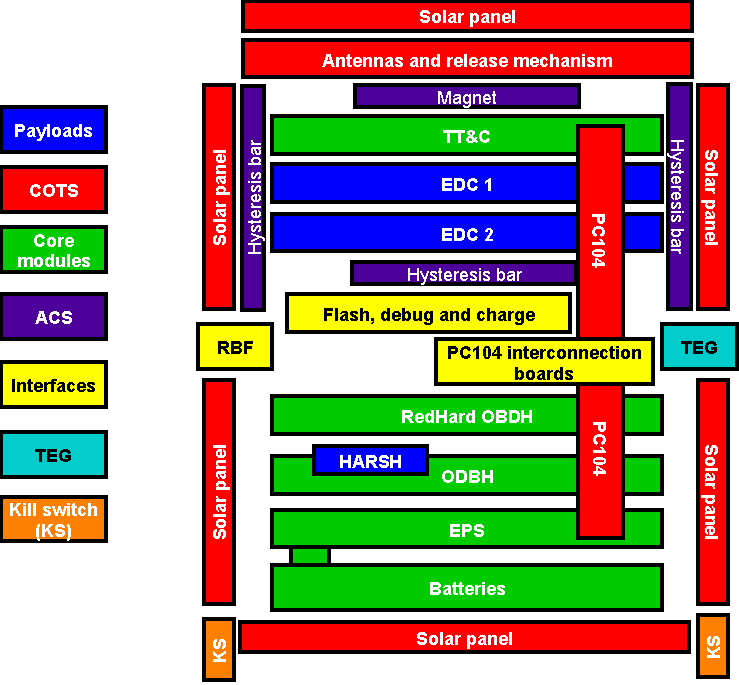
\includegraphics[width=0.7\textwidth]{figures/subsystems-positioning.pdf}
        \caption{Subsystems positioning.}
        \label{fig:subsystems-positioning}
    \end{center}
\end{figure}

%   TBD 
%   In \autoref{fig:datapath-diagram} there is a block diagram showing the satellite modules and the internal communication interfaces.

\subsection{Deployment Sequence}

The deployment sequence of the satellite is the routine to be executed just after the launch. The main objective of this operation is to the deploy the antennas and prepare the satellite to start its normal operation.

Just after the satellite is ejected from the deployer, the kill-switches enables the electric power and the three core modules execute the boot sequence (EPS, OBDH and TTC). The EPS module is ready to operate when the boot finishes. The OBDH and the TTC modules waits for a determined period before starting the normal execution.

As the OBDH and the TTC have access to the antenna module, both subsystem can control the deployment of the antennas. Following the CDS\nomenclature{\textbf{CDS}}{\textit{CubeSat Design Specification.}} specifications \cite{cds}, all CubeSats must wait 30 minutes to deploy the antennas and 45 minutes to transmit any RF signal. This way, the OBDH waits 45 minutes to send the deployment command to the antenna module. As redundancy, the TTC waits 55 minutes to execute the same operation.

The \autoref{fig:deployment-flowchart} has a flowchart that illustrates the deployment sequence of the service modules.

\begin{figure}[!ht]
    \begin{center}
        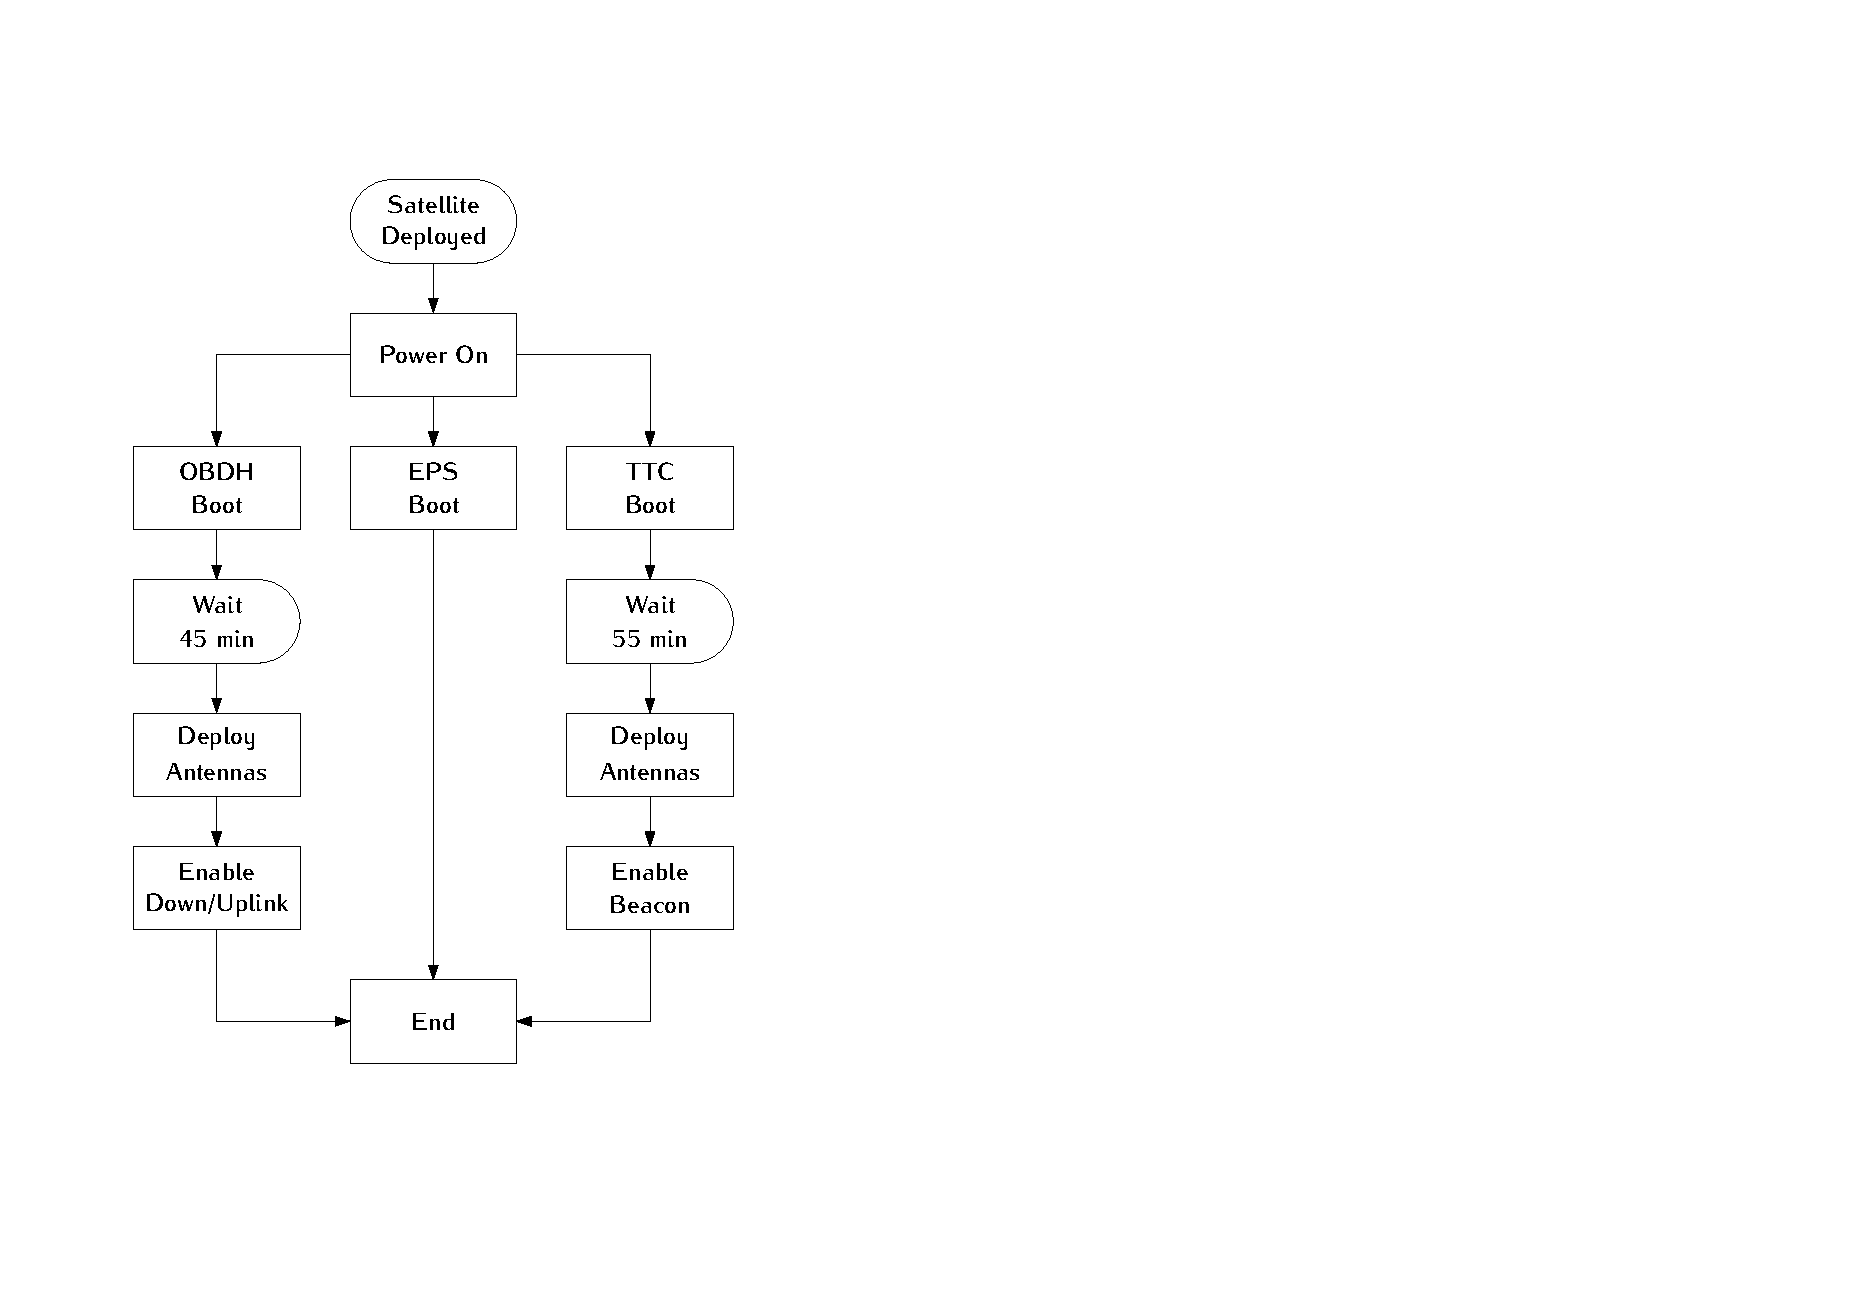
\includegraphics[width=0.5\textwidth]{figures/deployment-flowchart.pdf}
        \caption{Flowchart of the deployment sequence.}
        \label{fig:deployment-flowchart}
    \end{center}
\end{figure}

\subsection{Beacon Operation}

After the boot sequence of the beacon microcontroller, the operation of the beacon starts. The normal operation consist on reading the data from the EPS and the TTC modules, transmit the valid data (EPS or TTC package, in this order of priority), wait 60 seconds and repeat this sequence. The \autoref{fig:beacon-flowchart} has a flowchart of this behaviour.

\begin{figure}[!ht]
    \begin{center}
        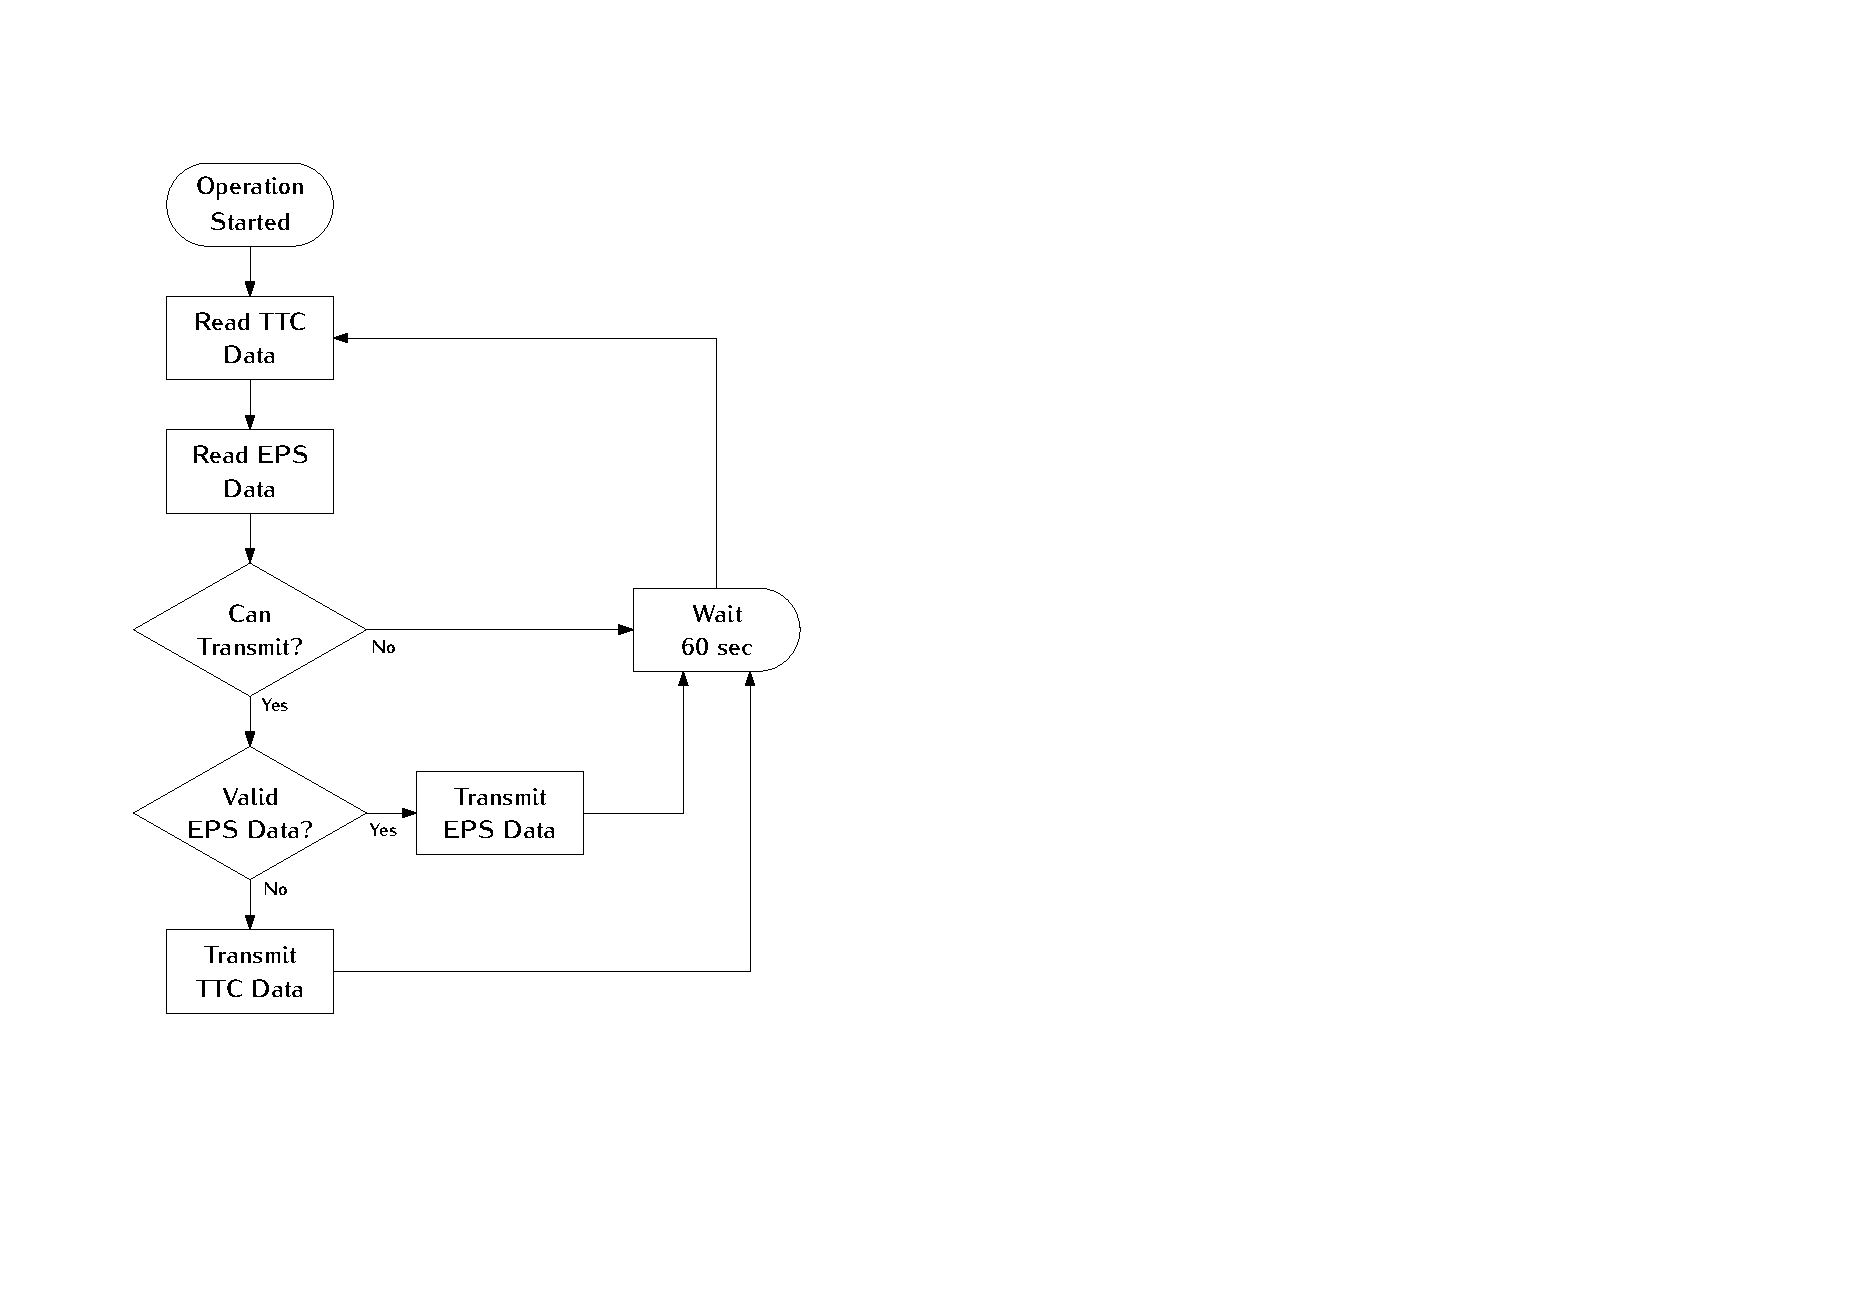
\includegraphics[width=0.55\textwidth]{figures/beacon-flowchart.pdf}
        \caption{Flowchart of the normal beacon operation.}
        \label{fig:beacon-flowchart}
    \end{center}
\end{figure}

\section{General Behaviour}

.

\section{Orbit Parameters and Analysis}

To define the orbit parameters and simulate the behaviour of the satellite during its operation, the GMAT\nomenclature{\textbf{GMAT}}{\textit{General Mission Analysis Tool.}} software was used \cite{gmat}. The orbit parameters was based on the FloripaSat-I TLE\nomenclature{\textbf{TLE}}{\textit{Two-Line Element.}}, but with a lower altitude. These parameters can be seen in \autoref{tab:orbit-parameters}.

\begin{table}[!h]
    \centering
    \begin{tabular}{lcc}
        \toprule[1.5pt]
        \textbf{Parameters} & \textbf{Value} & \textbf{Unit} \\
        \midrule
        Altitude                & 550           & km \\
        Eccentricity            & 0,0015051     & $^{\circ}$ \\
        Inclination             & 97,9750       & $^{\circ}$ \\
        RAAN                    & 85,5100       & $^{\circ}$ \\
        Arg. of Perigee (AOP)   & 194,87        & $^{\circ}$ \\
        TA                      & 99,8877       & $^{\circ}$ \\
        \bottomrule[1.5pt]
    \end{tabular}
    \caption{Initial orbit parameters (adapted from FloripaSat-I).}
    \label{tab:orbit-parameters}
\end{table}

The parameters of the simulation on GMAT was based on \cite{marino2016} and can be seen below:

\begin{itemize}
    \item Force model for gravitational field: ``\textit{Earth Gravitational Model 1996 (EGM96)}''
    \item Propagator: ``\textit{PrinceDorman78}''
    \item Drag coefficient: 2,2
    \item Drag atmosphere model: ``\textit{Mass Spectrometry and Incoherent Scatter (MSISE90)}''
    \item Epoch: 01 Jan 2022 11:59:28.000
\end{itemize}

The \autoref{fig:fsat2-gmat} shows the 3D representation of the FloripaSat-2 orbit simulation, \autoref{fig:fsat2-gmat-groundtrack} shows the ground track of the first day of operation.

\begin{figure}[!ht]
    \begin{center}
        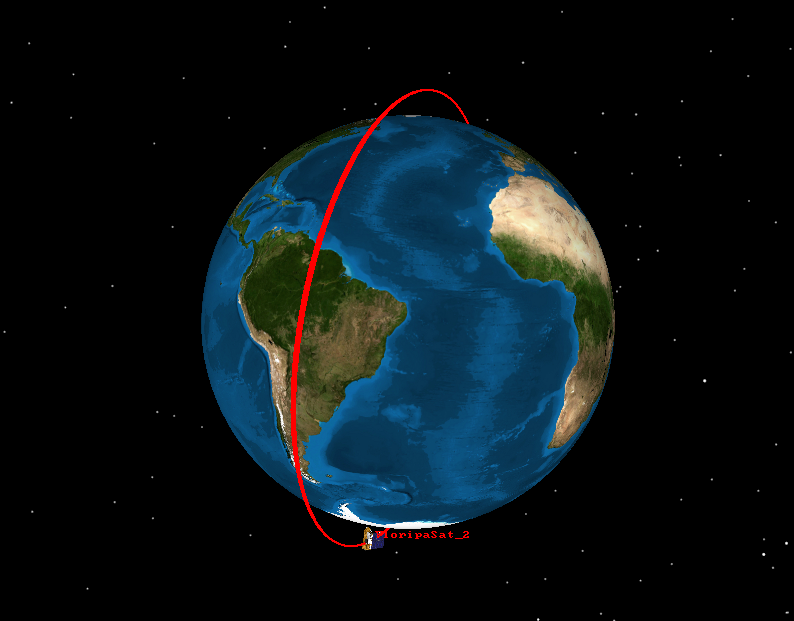
\includegraphics[width=0.6\textwidth]{figures/fsat2-gmat.png}
        \caption{FloripaSat-2 orbit simulation on GMAT.}
        \label{fig:fsat2-gmat}
    \end{center}
\end{figure}

\begin{figure}[!ht]
    \begin{center}
        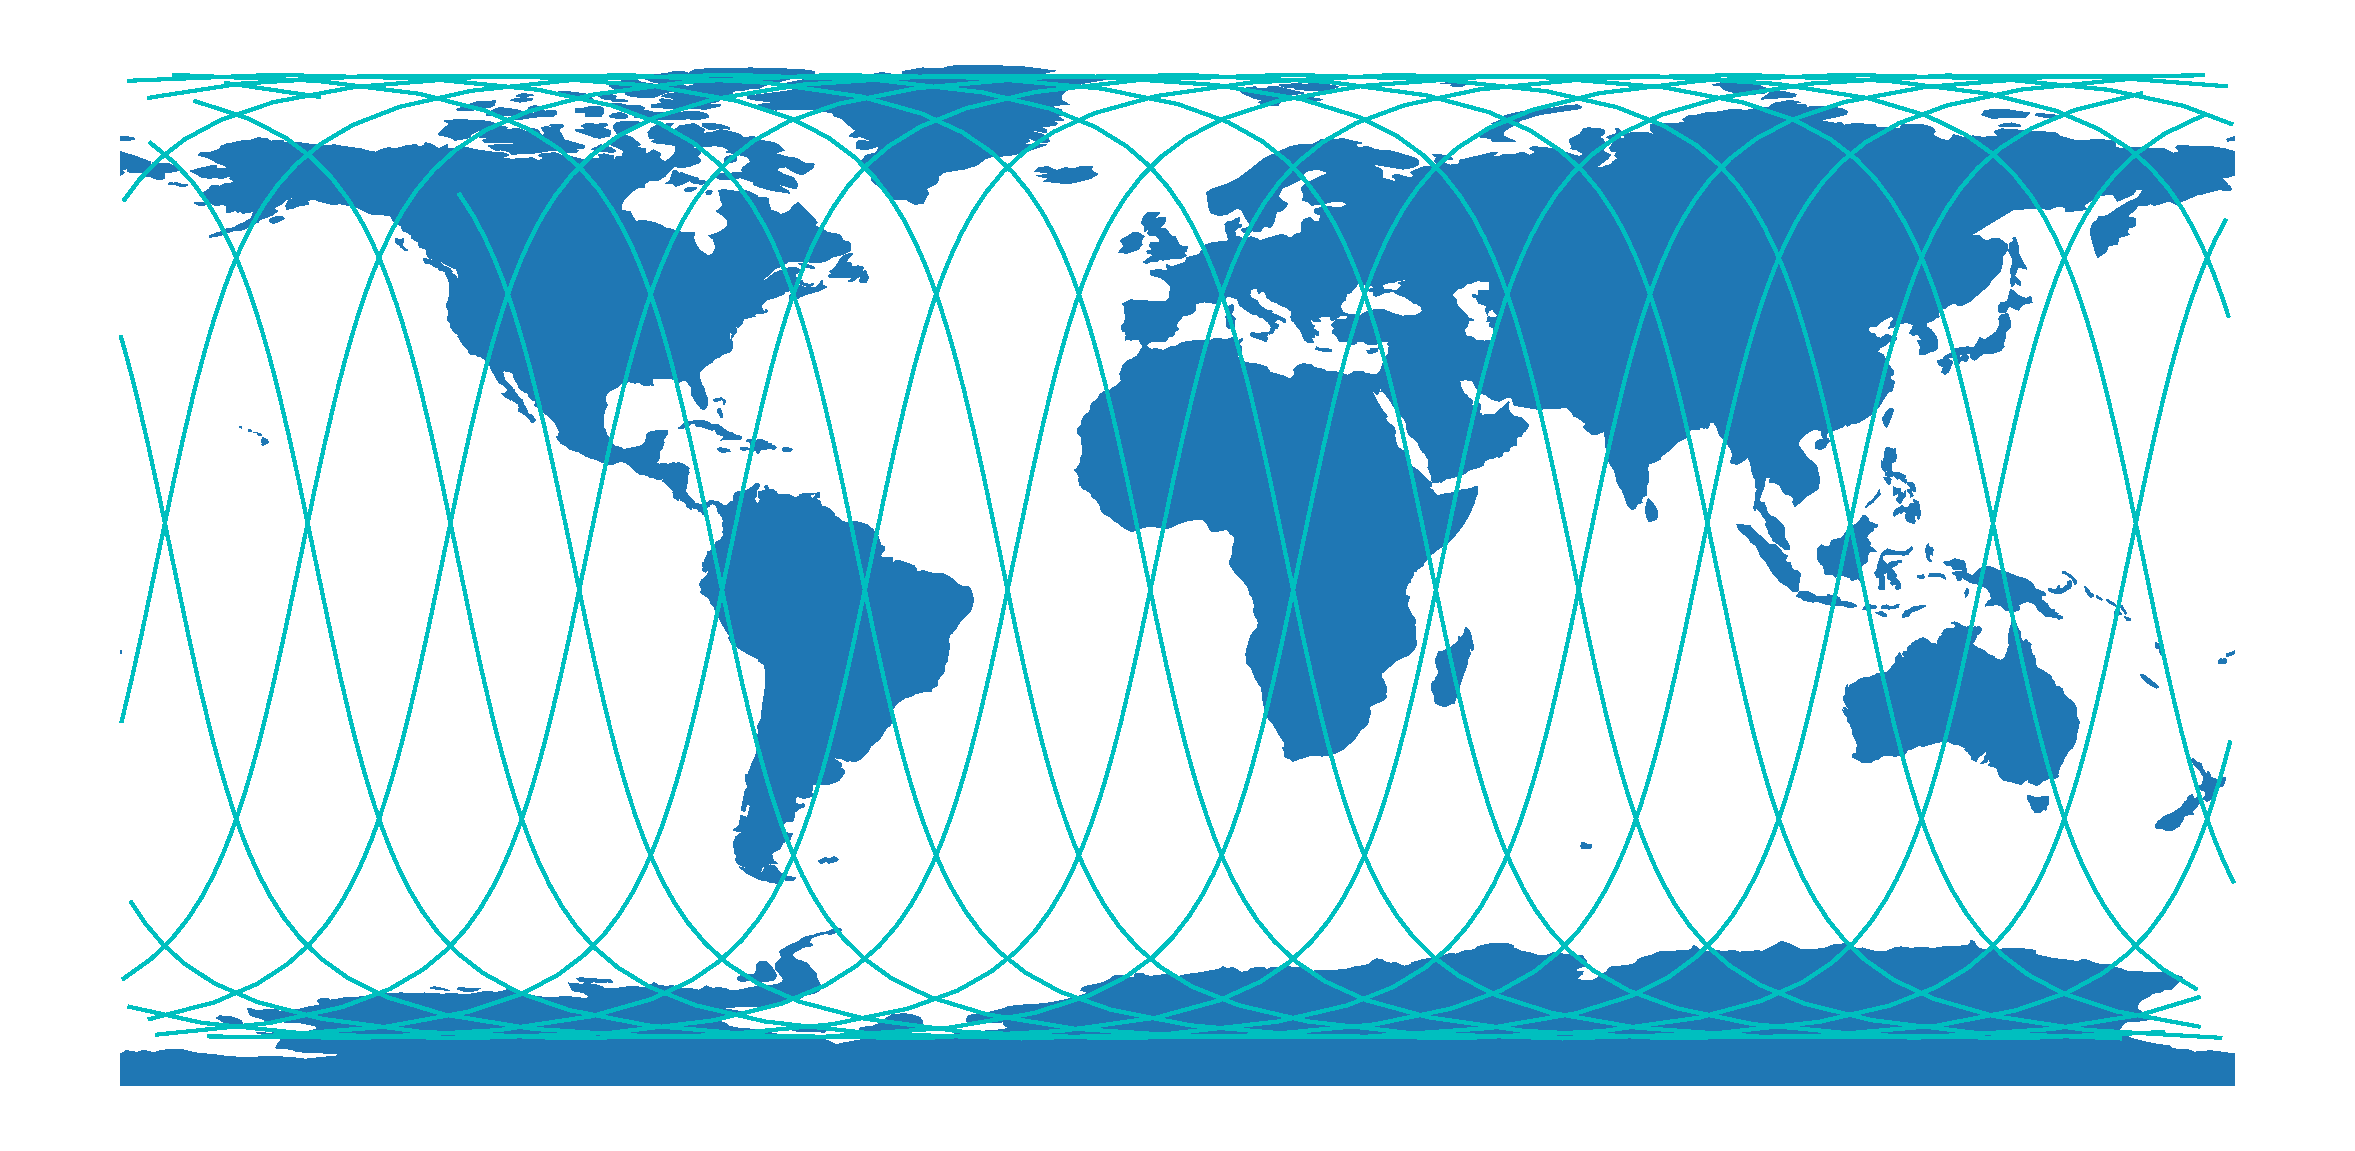
\includegraphics[width=\textwidth]{figures/fsat2-gmat-groundtrack.pdf}
        \caption{FloripaSat-2 simulated groundtrack.}
        \label{fig:fsat2-gmat-groundtrack}
    \end{center}
\end{figure}

The next sections present some analysis based on the results obtained on the simulations executed on GMAT.

The source files of the GMAT simulation are available in \cite{fsat2-mechanical}.

\subsection{Lifetime Analysis}

Considering the same parameters of FloripaSat-I, but with an initial altitude of 550 km, the simulations on GMAT showed that the satellite decays approximately in 2000 days ($\cong$ 5 years), as can be seen in \autoref{fig:lifetime-analysis}.

\begin{figure}[!ht]
    \begin{center}
        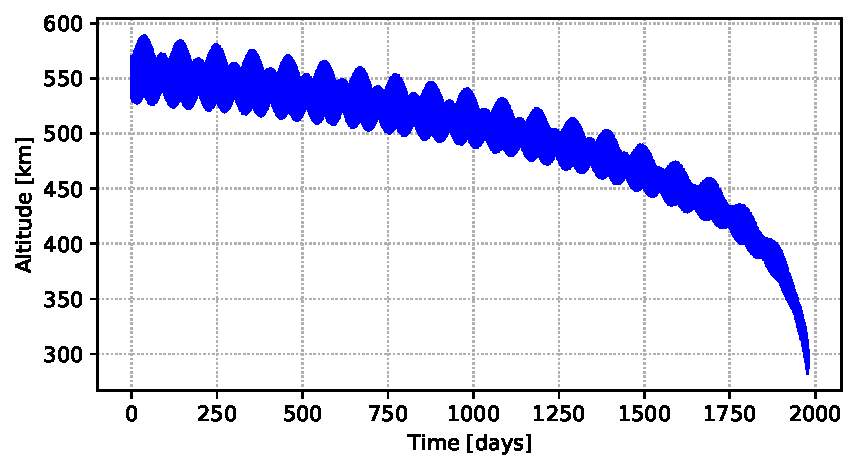
\includegraphics[width=\textwidth]{curves/lifetime.pdf}
        \caption{Lifetime analysis on GMAT.}
        \label{fig:lifetime-analysis}
    \end{center}
\end{figure}

\subsection{Ground Station Passes and Data Transfer Analysis}

Considering two ground stations, one at the SpaceLab installations in Florianópolis (27$^{\circ}$ 36' 00.9" S, 48$^{\circ}$ 31' 03.2" W) and other at the INPE/CRN installations in Natal (5$^{\circ}$ 50' 10.1" S, 35$^{\circ}$ 12' 27.5" W), both with a minimum elevation of 15$^{\circ}$, the following results were achieved during the simulations on GMAT (\autoref{tab:grs-contacts-analysis}).

\begin{table}[!h]
    \centering
    \begin{tabular}{lccc}
        \toprule[1.5pt]
        \textbf{Parameter} & \textbf{UFSC Station} & \textbf{INPE-RN Station} & \textbf{Unit} \\
        \midrule
        Minimum elevation to a valid contact    & 15    & 15    & $^{\circ}$ \\
        Number of contacts                      & 143   & 125   & - \\
        Minimum contact period                  & 24    & 34    & sec \\
        Maximum contact period                  & 395   & 394   & sec \\
        Average contact period                  & 303   & 298   & sec \\
        Total contact period                    & 43394 & 37205 & sec \\
        \bottomrule[1.5pt]
    \end{tabular}
    \caption{Ground station contacts analysis during the first 60 days of operation.}
    \label{tab:grs-contacts-analysis}
\end{table}

As can be seen from \autoref{tab:grs-contacts-analysis}, during the first 60 days of operation, considering the two main ground stations that will contact the satellite, the total contact period is 80599 seconds (43394 + 37205). With the data rate of the downlink/uplink as 4800 bps, this time period will allow a data transfer of 48359400 bytes (or 46,12 M$_{i}$B) between FloripaSat-2 and the Earth. Using the lifetime of the satellite from the previous analysis (2000 days), and an average data transfer per day of 805990 bits, the total theoretical raw data transfer during the whole operation of the satellite will be approximately 1,5 G$_{i}$B.

These values can be even bigger if a smaller minimum elevation is considered, or with more ground stations in other locations.

\section{Power Budget}

According to section 10.3 of \cite{larson2005}, the power budget of satellite can be determined through three steps:

\begin{enumerate}
    \item Prepare operating power budget
    \item Size the battery
    \item Estimate power degradation over mission life
\end{enumerate}

\subsection{Operating Power Budget}

\begin{table}[!h]
    \centering
    \begin{tabular}{lccccc}
        \toprule[1.5pt]
        \multirow{2}{*}{\textbf{Module}} & \multirow{2}{*}{\textbf{Voltage [V]}}    & \multicolumn{2}{c}{\textbf{Current [mA]}} & \multicolumn{2}{c}{\textbf{Power [mW]}} \\
                                         &                                          & \textbf{Min.} & \textbf{Max.}             & \textbf{Min.} & \textbf{Max.} \\
        \midrule
        OBDH                & 3,3   & TBD   & TBD   & TBD   & TBD \\
        TTC ($\mu$C)        & 3,3   & TBD   & TBD   & TBD   & TBD \\
        TTC (radio module)  & 5     & TBD   & 650   & TBD   & 3250 \\
        EPS (digital part)  & 3,3   & TBD   & TBD   & TBD   & TBD \\
        EPS (heater)        & 3,3   & TBD   & TBD   & TBD   & TBD \\
        Antenna module      & 3,3   & TBD   & TBD   & TBD   & TBD \\
        Payload EDC         & 5     & 250   & 250   & 1250  & 1250 \\
        Payload-X           & 5     & TBD   & TBD   & TBD   & TBD \\
        Payload Harsh       & 3,3   & TBD   & TBD   & TBD   & TBD \\
        \bottomrule[1.5pt]
    \end{tabular}
    \caption{Power requirements of the subsystems and payloads of the satellite.}
    \label{tab:power-requirements}
\end{table}

Assumptions:

\begin{itemize}
    \item One of the EDC payload is always off (cold redundancy).
    \item The Payload-X and the Harsh payload are turned on just during limited periods.
\end{itemize}

\subsection{Battery Sizing}

.

\subsection{Power Degradation Over Mission Life}

\begin{itemize}
    \item Solar panels degradation
    \item Battery degradation
\end{itemize}

\section{Link Budget}

The link budget of all radio links of the satellite is available in \autoref{tab:link-budget-results}.

\begin{table}[!h]
    \centering
    \begin{tabular}{L{0.3\textwidth}ccccc}
        \toprule[1.5pt]
        \textbf{Variable} & \textbf{Beacon} & \textbf{Downlink} & \textbf{Uplink} & \textbf{Uplink (Payload)} & \textbf{Unit}\\
        \midrule
        Frequency                       & 145,97    & 436,9     & 436,9     & 401,635   & MHz \\
        Modulation                      & GMSK      & GMSK      & GMSK      & BPSK      & - \\
        Protocol                        & NGHam     & NGHam     & NGHam     & SBCD      & - \\
        Transmit power                  & 30        & 30        & 47        & ??        & dBm \\
        FSPL                            & 144,8     & 154,3     & 154,3     & ??        & dB \\
        Other losses                    & 5         & 5         & 7         & 5         & dB \\
        Receive antenna gain            & 12        & 15.5      & 0         & 0         & dBi \\
        Receiver noise temp.            &           &           &           &           & K \\
        Antenna noise temp.             &           &           &           &           & K \\
        System noise temp.              &           &           &           &           & K \\
        Data rate                       & 1200      & 4800      & 4800      & 400       & bps \\
        Received SNR                    & 30,87     & 17,35     & 31,60     & ??        & dB \\
        SNR required for $10^{-5}$ BER*  & 9,6       & 9,6       & 9,6       & 9,6       & dB \\
        Link margin                     & $\leq$ 21,27 & $\leq$ 7,75 & $\leq$ 22 & $\leq$ ?? & dB \\
        \bottomrule[1.5pt]
    \end{tabular}
    \caption{Link budget results.}
    \label{tab:link-budget-results}
\end{table}

All equations and steps used to obtain the results of \autoref{tab:link-budget-results} are available in \autoref{anx:link-budget}.

\section{PC-104 Bus}

To electrically connect all the satellite modules, a PC-104 bus standard is being used. This bus is composed by 104 lines disposed by four rows of 26 pins each (with a vertical and horizontal pitch of 2,54 mm).

Using the \autoref{fig:pc104-ref-diagram} as reference, all used positions and signals of the PC-104 bus are presented in \autoref{tab:pc104-pinout}. The \autoref{tab:pc104-signals} describes each signal and which modules are connected to them.

\begin{figure}[!ht]
    \begin{center}
        \includegraphics[width=0.5\textwidth]{figures/pc104-diagram}
        \caption{Reference diagram of the PC-104 bus (top view of a generic module).}
        \label{fig:pc104-ref-diagram}
    \end{center}
\end{figure}

\begin{table}[!h]
    \centering
    \begin{tabular}{cllll}
        \toprule[1.5pt]
        \textbf{Pin Row}   & \textbf{H1 Odd}  & \textbf{H1 Even} & \textbf{H2 Odd} & \textbf{H2 Even} \\
        \midrule
        1-2                & -                & -                & -               & -                \\
        3-4                & -                & -                & EDC\_1\_EN      & EDC\_2\_EN       \\
        5-6                & -                & -                & BE\_UART\_RX    & -                \\
        7-8                & RA\_GPIO\_0      & RA\_GPIO\_1      & BE\_UART\_TX    & GPIO\_0          \\
        9-10               & RA\_GPIO\_2      & BE\_EN           & -               & -                \\
        11-12              & RA\_RESET        & RA\_EN           & BE\_SPI\_MOSI   & BE\_SPI\_CLK     \\
        13-14              & -                & -                & BE\_SPI\_CS     & BE\_SPI\_MISO    \\
        15-16              & -                & -                & -               & -                \\
        17-18              & EDC\_UART\_RX/TX & PLX\_EN          & -               & GPIO\_1          \\
        19-20              & EDC\_UART\_TX/RX & GPIO\_2          & -               & GPIO\_3          \\
        21-22              & -                & -                & -               & GPIO\_4          \\
        23-24              & -                & -                & -               & -                \\
        25-26              & -                & -                & PL\_VCC         & PL\_VCC          \\
        27-28              & -                & -                & TTC\_VCC        & TTC\_VCC         \\
        29-30              & GND              & GND              & GND             & GND              \\
        31-32              & GND              & GND              & GND             & GND              \\
        33-34              & -                & -                & -               & -                \\
        35-36              & RA\_SPI\_CLK     & -                & ANT\_VCC        & ANT\_VCC         \\
        37-38              & RA\_SPI\_MISO    & -                & -               & -                \\
        39-40              & RA\_SPI\_MOSI    & RA\_SPI\_CS      & -               & -                \\
        41-42              & PL\_I2C\_SDA     & -                & -               & GPIO\_5          \\
        43-44              & PL\_I2C\_SCL     & -                & -               & -                \\
        45-46              & OBDH\_VCC        & OBDH\_VCC        & BAT\_VCC        & BAT\_VCC         \\
        47-48              & PL\_VCC          & PL\_VCC          & -               & -                \\
        49-50              & RA\_VCC          & RA\_VCC          & EPS\_I2C\_SDA   & -                \\
        51-52              & BE\_VCC          & BE\_VCC          & EPS\_I2C\_SCL   & -                \\
        \bottomrule[1.5pt]
    \end{tabular}
    \caption{PC-104 bus pinout.}
    \label{tab:pc104-pinout}
\end{table}

\begin{table}[!h]
    \centering
    \begin{tabular}{lL{0.18\textwidth}L{0.17\textwidth}L{0.33\textwidth}}
        \toprule[1.5pt]
        \textbf{Signal}  & \textbf{Pin(s)} & \textbf{Used By}     & \textbf{Description} \\
        \midrule
        GND              & H1-29/30/31/32, H2-29/30/31/32 & All   & Ground reference \\
        BAT\_VCC         & H2-45, H2-46    & EPS                  & Battery terminals (+) \\
        ANT\_VCC         & H2-35, H2-36    & EPS, ANT             & Antenna power supply (3.3 V) \\
        OBDH\_VCC        & H1-45, H1-46    & EPS, OBDH            & OBDH power supply (3.3 V) \\
        TTC\_VCC         & H2-27, H2-28    & EPS, TTC             & TTC power supply (3.3 V) \\
        PL\_VCC          & H1-47/48, H2-25/26 & EPS, EDC 1/2, Payload X & Payloads power supply (5 V) \\
        RA\_VCC          & H1-49, H1-50    & EPS, TTC             & Main radio power supply (5 V) \\
        BE\_VCC          & H1-51, H1-52    & EPS, TTC             & Beacon power supply (6 V) \\
        RA\_SPI\_CLK     & H1-35           & OBDH, TTC            & CLK signal of the main radio SPI bus \\
        RA\_SPI\_MISO    & H1-37           & OBDH, TTC            & MISO signal of the main radio SPI bus \\
        RA\_SPI\_MOSI    & H1-39           & OBDH, TTC            & MOS signal of the main radio SPI bus \\
        RA\_SPI\_CS      & H1-40           & OBDH, TTC            & CS signal of the main radio SPI bus \\
        EPS\_I2C\_SDA    & H2-49           & OBDH, EPS            & SDA signal of the EPS I2C bus \\
        EPS\_I2C\_SCL    & H2-51           & OBDH, EPS            & SCL signal of the EPS I2C bus \\
        BE\_UART\_RX     & H2-5            & EPS, TTC             & EPS TX, Beacon RX (UART bus) \\
        BE\_UART\_TX     & H2-7            & EPS, TTC             & EPS RX, Beacon TX (UART bus) \\
        EDC\_UART\_TX/RX & H1-25           & OBDH, EDC 1/2        & OBDH TX, EDCs RX (UART bus) \\
        EDC\_UART\_RX/TX & H1-27           & OBDH, EDC 1/2        & OBDH RX, EDCs TX (UART bus) \\
        BE\_EN           & H1-10           & EPS, TTC             & Beacon radio power enable \\
        RA\_EN           & H1-12           & EPS, OBDH            & Main radio power enable \\
        EDC\_1\_EN       & H2-3            & OBDH, EDC 1          & EDC 1 enable signal \\
        EDC\_2\_EN       & H2-4            & OBDH, EDC 2          & EDC 2 enable signal \\
        PLX\_EN          & H1-18           & OBDH, Payload X      & Payload X enable (GPIO) \\
        PL\_I2C\_SDA     & H1-41           & OBDH, Payload X      & SDA signal of the payload I2C bus \\
        PL\_I2C\_SCL     & H1-43           & OBDH, Payload X      & SCL signal of the payload I2C bus \\
        GPIO\_N          & H1-20, H2-8/18/20/22/42  & OBDH        & GPIO pin (not used) \\
        \bottomrule[1.5pt]
    \end{tabular}
    \caption{PC-104 bus signal description.}
    \label{tab:pc104-signals}
\end{table}

The distribution pattern of pins adopted in this project is a mix of multiple different patterns from CubeSat modules manufacturers, like GomSpace, ISIS and Endurosat. Some pins are positioned to attend specific project requirements, and it is possible that the adopted pattern is not totally compatible to some commercial modules.

Beyond the PC-104 bus, there are some signals connected directly by wires and cables, like the control and power pins of the antenna module, the battery charger and the programming ports.

\section{Telecommunication}

\begin{landscape}
    \begin{table}[ht]
        \centering
        \begin{tabular}{llccccc}
            \toprule[1.5pt]
            \multirow{2}{*}{\textbf{Link}} & \multirow{2}{*}{\textbf{Packet Name}} & \multicolumn{4}{c}{\textbf{Payload}} & \multirow{2}{*}{\textbf{Access}} \\
            \cmidrule{3-6}
                                      &                       & \textbf{ID}  & \textbf{Source Callsign}   & \textbf{Data (up to 220 bytes)}            & \textbf{Size (bytes)} & \\
            \midrule
            \multirow{2}{*}{Beacon}   & EPS data              & 00h & \multirow{2}{*}{``0'' + ``PY0EFS''} & EPS data                                   & 58                    & Public \\
                                      & TTC Data              & 01h &                                     & TTC data                                   & 18                    & Public \\
            \midrule
            \multirow{8}{*}{Downlink} & General telemetry     & 20h & \multirow{8}{*}{``0'' + ``PY0EFS''} & OBDH/EPS data                              & 75                    & Public \\
                                      & Ping answer           & 21h &                                     & Requester callsign                         & 15                    & Public \\
                                      & Data request answer   & 22h &                                     & Req. callsign + data                       & 15 to 155             & Public \\
                                      & Message broadcast     & 23h &                                     & Req. + dst. callsign + message             & 22 to 60              & Public \\
                                      & Hibernation feedback  & 24h &                                     & Req. callsign + hibernation in hours       & 17                    & Public \\
                                      & EDC info              & 25h &                                     & PTT decoder + HK info + system state       & 79                    & Public \\
                                      & EDC samples           & 26h &                                     & Timestamp + pkt. counter + samples         & 219                   & Public \\
                                      & TC feedback           & 27h &                                     & Req. callsign + TC packet ID + timestamp   & 13                    & Public \\
            \midrule
            \multirow{12}{*}{Uplink}  & Ping Request          & 40h & \multirow{12}{*}{Any Callsign}      & None                                       & 8                     & Public \\
                                      & Data Request          & 41h &                                     & Data flags + count + origin + offset       & 16                    & Public \\
                                      & Broadcast Message     & 42h &                                     & Dst. callsign + message                    & 15 to 46              & Public \\
                                      & Enter hibernation     & 43h &                                     & Req. callsign + hibernation in hours + key & 29                    & Private \\
                                      & Leave hibernation     & 44h &                                     & Command key                                & 16                    & Private \\
                                      & Activate module       & 45h &                                     & Module ID + Command key                    & 17                    & Private \\
                                      & Deactivate module     & 46h &                                     & Module ID + Command key                    & 17                    & Private \\
                                      & Activate Payload      & 47h &                                     & Payload ID + Command key                   & 17                    & Private \\
                                      & Deactivate Payload    & 48h &                                     & Payload ID + Command key                   & 17                    & Private \\
                                      & Get EDC info          & 49h &                                     & Command key                                & 16                    & Private \\
            \bottomrule[1.5pt]
        \end{tabular}
        \caption{Telecommunication packets and their content.}
        \label{tab:packets-struct}
    \end{table}
\end{landscape}

\begin{table}[ht]
    \centering
    \begin{tabular}{lcL{0.53\textwidth}c}
        \toprule[1.5pt]
        \textbf{Packet} & \textbf{Position} & \textbf{Content} & \textbf{Length [bytes]} \\
        \midrule
        \multirow{22}{*}{EPS data} & 0  & Packet ID (00h)                       & 1 \\
                                   & 1  & Source callsign (``0PY0EFS'')         & 7 \\
                                   & 8  & Timestamp in ms                       & 4 \\
                                   & 12 & Battery cell 1 voltage in mV          & 2 \\
                                   & 14 & Battery cell 2 voltage in mV          & 2 \\
                                   & 16 & Battery current in mA                 & 2 \\
                                   & 18 & Battery charge in mAh                 & 2 \\
                                   & 20 & Battery cell 1 temperature in K       & 2 \\
                                   & 22 & Battery cell 2 temperature in K       & 2 \\
                                   & 24 & Battery monitor temperature in K      & 2 \\
                                   & 26 & Solar panel voltage in mV (-Y and +X) & 2 \\
                                   & 28 & Solar panel voltage in mV (-X and +Z) & 2 \\
                                   & 30 & Solar panel voltage in mV (-Z and +Y) & 2 \\
                                   & 32 & Solar panel current in mA (-Y)        & 2 \\
                                   & 34 & Solar panel current in mA (+Y)        & 2 \\
                                   & 36 & Solar panel current in mA (-X)        & 2 \\
                                   & 38 & Solar panel current in mA (+X)        & 2 \\
                                   & 40 & Solar panel current in mA (-Z)        & 2 \\
                                   & 42 & Solar panel current in mA (+Z)        & 2 \\
                                   & 44 & Temperature of the EPS $\mu$C in K    & 2 \\
        \cmidrule{4-4}
                                   &    &                                       & 46 \\
        \midrule
        \multirow{9}{*}{TTC data}  & 0  & Packet ID (01h)                       & 1 \\
                                   & 1  & Source callsign (``0PY0EFS'')         & 7 \\
                                   & 8  & Timestamp in ms                       & 4 \\
                                   & 12 & Temperature of the TTC $\mu$C in K    & 2 \\
                                   & 14 & Reset counter                         & 2 \\
                                   & 16 & Last reset cause                      & 1 \\
                                   & 15 & Temperature of the beacon radio in K  & 2 \\
        \cmidrule{4-4}
                                   &    &                                       & 19 \\
        \bottomrule[1.5pt]
    \end{tabular}
    \caption{Beacon packets.}
    \label{tab:beacon-packets}
\end{table}

\begin{longtable}[c]{lcL{0.4\textwidth}c}
    \toprule[1.5pt]
    \textbf{Packet} & \textbf{Position} & \textbf{Content} & \textbf{Length [bytes]} \\
    \midrule
    \multirow{39}{*}{General telemetry}     & 0  & Packet ID (20h)                              & 1 \\
                                            & 1  & Source callsign (``0PY0EFS'')                & 7 \\
                                            & 8  & Time counter in milliseconds                 & 4 \\
                                            & 12 & Temperature of the OBDH $\mu$C in Kelvin     & 2 \\
                                            & 14 & Input current of the OBDH in mA              & 2 \\
                                            & 16 & Input voltage of the OBDH in mV              & 2 \\
                                            & 18 & Last reset cause of the OBDH                 & 1 \\
                                            & 19 & Reset counter of the OBDH                    & 2 \\
                                            & 21 & Last valid telecommand (uplink packet ID)    & 1 \\
                                            & 22 & Temperature of the radio in Kelvin           & 2 \\
                                            & 24 & RSSI of the last valid telecommand           & 2 \\
                                            & 26 & Temperature of the antenna in Kelvin         & 2 \\
                                            & 28 & Antenna status                               & 2 \\
                                            & 30 & Payloads status                              & 1 \\
                                            & 31 & Temperature of the EPS $\mu$C in K           & 2 \\
                                            & 33 & EPS circuitry and Beacon MCU current in mA   & 2 \\
                                            & 35 & Last reset cause of the EPS                  & 1 \\
                                            & 36 & Reset counter (EPS)                          & 2 \\
                                            & 38 & -Y and +X sides solar panel voltage in mV    & 2 \\
                                            & 40 & -X and +Z sides solar panel voltage in mV    & 2 \\
                                            & 42 & -Z and +Y sides solar panel voltage in mV    & 2 \\
                                            & 44 & -Y side solar panel current in mA            & 2 \\
                                            & 46 & +Y side solar panel current in mA            & 2 \\
                                            & 48 & -X side solar panel current in mA            & 2 \\
                                            & 50 & +X side solar panel current in mA            & 2 \\
                                            & 52 & -Z side solar panel current in mA            & 2 \\
                                            & 54 & +Z side solar panel current in mA            & 2 \\
                                            & 55 & MPPT 1 duty cycle in \%                      & 1 \\
                                            & 56 & MPPT 2 duty cycle in \%                      & 1 \\
                                            & 57 & MPPT 3 duty cycle in \%                      & 1 \\
                                            & 59 & Main power bus voltage in mV                 & 2 \\
                                            & 61 & Batteries voltage in mV                      & 2 \\
                                            & 63 & Batteries current in mA                      & 2 \\
                                            & 65 & Batteries average current in mA              & 2 \\
                                            & 67 & Batteries accumulated current in mA          & 2 \\
                                            & 69 & Batteries charge in mAh                      & 2 \\
                                            & 71 & Battery monitor IC temperature in K          & 2 \\
                                            & 73 & Battery heater 1 duty cycle in \%            & 1 \\
                                            & 74 & Battery heater 2 duty cycle in \%            & 1 \\
    \cmidrule{4-4}
                                            &    &                                              & 75 \\
    \multirow{3}{*}{Ping answer}            & 0  & Packet ID (21h)                      & 1 \\
                                            & 1  & Source callsign (``0PY0EFS'')        & 7 \\
                                            & 8  & Requester callsign                   & 7 \\
    \cmidrule{4-4}
                                            &    &                                      & 15 \\
    \multirow{3}{*}{Data request answer}    & 0  & Packet ID (22h)                      & 1 \\
                                            & 1  & Source callsign (``0PY0EFS'')        & 7 \\
                                            & 8  & Requester callsign                   & 7 \\
    \cmidrule{4-4}
                                            &    &                                      & 15 \\
    \multirow{5}{*}{Message broadcast}      & 0  & Packet ID (23h)                      & 1 \\
                                            & 1  & Source callsign (``0PY0EFS'')        & 7 \\
                                            & 8  & Requester callsign                   & 7 \\
                                            & 15 & Destination callsign                 & 7 \\
                                            & 22 & Message                              & up to 38 \\
    \cmidrule{4-4}
                                            &    &                                      & 22 to 60 \\
    \multirow{4}{*}{Hibernation feedback}   & 0  & Packet ID (24h)                      & 1 \\
                                            & 1  & Source callsign (``0PY0EFS'')        & 7 \\
                                            & 8  & Requester callsign                   & 7 \\
                                            & 15 & Hibernation in hours                 & 2 \\
    \cmidrule{4-4}
                                            &    &                                      & 17 \\
    \multirow{22}{*}{EDC info}              & 0  & Packet ID (25h)                      & 1 \\
                                            & 1  & Source callsign (``0PY0EFS'')        & 7 \\
                                            & 8  & PTT signal receiving time            & 4 \\
                                            & 12 & Error code                           & 1 \\
                                            & 13 & Carrier frequency                    & 2 \\
                                            & 15 & Carrier amplitude at ADC interface output & 2 \\
                                            & 17 & User message length in bytes         & 1 \\
                                            & 18 & ARGOS-2 PTT-A2 user message          & 35 \\
                                            & 53 & Current time since J2000 epoch       & 4 \\
                                            & 57 & Elapsed time since last reset        & 4 \\
                                            & 61 & System current supply in mA          & 2 \\
                                            & 63 & System voltage supply in mV          & 2 \\
                                            & 64 & EDC board temperature                & 1 \\
                                            & 65 & RF front end LO                      & 1 \\
                                            & 66 & RMS level at front-end output        & 2 \\
                                            & 68 & Generated PTT packages since last initialization & 1 \\
                                            & 69 & Max                                  & 1 \\
                                            & 70 & Memory error count                   & 1 \\
                                            & 71 & Current time                         & 4 \\
                                            & 75 & Number of PTT package available for reading & 1 \\
                                            & 76 & PTT decoder task status              & 1 \\
                                            & 77 & ADC sampler state                    & 1 \\
    \cmidrule{4-4}
                                            &    &                                      & 78 \\
    \multirow{9}{*}{EDC samples}            & 0  & Packet ID (26h)                      & 1 \\
                                            & 1  & Source callsign (``0PY0EFS'')        & 7 \\
                                            & 8  & Elapsed time since J2000 epoch       & 4 \\
                                            & 12 & ADC sample packet number             & 1 \\
                                            & 13 & First ADC I-sample                   & 2 \\
                                            & 15 & First ADC Q-sample                   & 2 \\
                                            & ... & ...                                 & ... \\
                                            & 213 & N ADC I-sample                      & 2 \\
                                            & 215 & N ADC Q-sample                      & 2 \\
    \cmidrule{4-4}
                                            &    &                                      & 217 \\
    \bottomrule[1.5pt]
    \caption{Downlink packets.}
    \label{tab:downlink-packets}
\end{longtable}

\begin{longtable}[c]{lcL{0.4\textwidth}c}
    \toprule[1.5pt]
    \textbf{Packet} & \textbf{Position} & \textbf{Content} & \textbf{Length [bytes]} \\
    \midrule
    \multirow{2}{*}{Ping request}       & 0  & Packet ID (40h)                      & 1 \\
                                        & 1  & Ground station callsign              & 7 \\
    \cmidrule{4-4}
                                        &    &                                      & 8 \\
    \multirow{2}{*}{Data request}       & 0  & Packet ID (41h)                      & 1 \\
                                        & 1  & Ground station callsign              & 7 \\
    \cmidrule{4-4}
                                        &    &                                      & 8 \\
    \multirow{4}{*}{Broadcast message}  & 0  & Packet ID (42h)                      & 1 \\
                                        & 1  & Ground station callsign              & 7 \\
                                        & 8  & Destination callsign                 & 7 \\
                                        & 15 & Message                              & up to 38 \\
    \cmidrule{4-4}
                                        &    &                                      & up to 53 \\
    \multirow{4}{*}{Enter hibernation}  & 0  & Packet ID (43h)                      & 1 \\
                                        & 1  & Ground station callsign              & 7 \\
                                        & 8  & Hibernation in hours                 & 2 \\
                                        & 10 & Command key                          & 8 \\
    \cmidrule{4-4}
                                        &    &                                      & 18 \\
    \multirow{3}{*}{Leave hibernation}  & 0  & Packet ID (44h)                      & 1 \\
                                        & 1  & Ground station callsign              & 7 \\
                                        & 8  & Command key                          & 8 \\
    \cmidrule{4-4}
                                        &    &                                      & 16 \\
    \multirow{4}{*}{Activate module}    & 0  & Packet ID (45h)                      & 1 \\
                                        & 1  & Ground station callsign              & 7 \\
                                        & 8  & Module ID                            & 1 \\
                                        & 9  & Command key (one for each module)    & 8 \\
    \cmidrule{4-4}
                                        &    &                                      & 17 \\
    \multirow{4}{*}{Deactivate module}  & 0  & Packet ID (46h)                      & 1 \\
                                        & 1  & Ground station callsign              & 7 \\
                                        & 8  & Module ID                            & 1 \\
                                        & 9  & Command key (one for each module)    & 8 \\
    \cmidrule{4-4}
                                        &    &                                      & 17 \\
    \multirow{4}{*}{Activate Payload}   & 0  & Packet ID (47h)                      & 1 \\
                                        & 1  & Ground station callsign              & 7 \\
                                        & 8  & Payload ID                           & 1 \\
                                        & 9  & Command key (one for each payload)   & 8 \\
    \cmidrule{4-4}
                                        &    &                                      & 17 \\
    \multirow{4}{*}{Deactivate Payload} & 0  & Packet ID (48h)                      & 1 \\
                                        & 1  & Ground station callsign              & 7 \\
                                        & 8  & Payload ID                           & 1 \\
                                        & 9  & Command key (one for each payload)   & 8 \\
    \cmidrule{4-4}
                                        &    &                                      & 17 \\
    \multirow{2}{*}{Get EDC info}       & 0  & Packet ID (49h)                      & 1 \\
                                        & 1  & Ground station callsign              & 7 \\
    \cmidrule{4-4}
                                        &    &                                      & 8 \\
    \bottomrule[1.5pt]
    \caption{Uplink packets.}
    \label{tab:uplink-packets}
\end{longtable}

\subsection{Operation Licenses}

.
